%=======================================================================
%  Foundations -- UML diagrams rendered in TikZ
%  CSE 360 Team Project
%
%  PURPOSE
%  -------
%  This document draws every diagram so you can see it, then redraw it
%  in Astah. It is a visual reference, not the deliverable -- main.tex
%  is the deliverable, and it has a slot for each Astah export.
%
%  DEPENDENCIES
%  ------------
%  Only tikz and its standard libraries. No tikz-uml, no pgf-umlsd.
%  This compiles on any complete TeX installation and on Overleaf.
%
%  IF SOMETHING FAILS TO COMPILE
%  -----------------------------
%  Each diagram is self-contained between its own banner comment, so a
%  broken one can be commented out without affecting the others.
%=======================================================================

\documentclass[11pt,a4paper]{article}

\usepackage[T1]{fontenc}
\usepackage[utf8]{inputenc}
\usepackage[margin=0.8in,landscape]{geometry}
\usepackage{tikz}
\usepackage{float}
\usepackage{xcolor}
\usepackage{caption}

\usetikzlibrary{positioning}
\usetikzlibrary{shapes.multipart}
\usetikzlibrary{arrows.meta}
\usetikzlibrary{calc}
\usetikzlibrary{fit}
\usetikzlibrary{backgrounds}
\usetikzlibrary{automata}

\definecolor{accent}{HTML}{4338CA}
\definecolor{muted}{HTML}{667085}
\definecolor{soft}{HTML}{EEF2FF}
\definecolor{band}{HTML}{F4F5F8}

%-----------------------------------------------------------------------
% Shared styles
%-----------------------------------------------------------------------
\tikzset{
  % A UML class box: name / attributes / operations
  umlclass/.style={
    draw=black!70, fill=white, rectangle split, rectangle split parts=3,
    rectangle split draw splits=true, align=left, font=\scriptsize,
    inner sep=4pt, text width=#1},
  % A class box with only a name and one compartment
  umlclasstwo/.style={
    draw=black!70, fill=white, rectangle split, rectangle split parts=2,
    rectangle split draw splits=true, align=left, font=\scriptsize,
    inner sep=4pt, text width=#1},
  % A package
  pkg/.style={
    draw=black!70, fill=soft, rectangle, align=center,
    font=\scriptsize, inner sep=4pt, minimum height=8mm, text width=#1},
  % A plain node for navigation graphs
  page/.style={
    draw=black!60, fill=white, rounded corners=2pt, align=center,
    font=\scriptsize, inner sep=3pt, minimum height=6mm, text width=#1},
  % Relationships
  uses/.style={-{Stealth[length=2mm]}, draw=black!60, dashed},
  calls/.style={-{Stealth[length=2mm]}, draw=black!70},
  msg/.style={-{Stealth[length=2mm]}, draw=black!80},
  ret/.style={-{Stealth[length=2mm]}, draw=black!50, dashed},
  lbl/.style={font=\scriptsize, inner sep=1.5pt, fill=white},
  band/.style={draw=none, fill=band, rounded corners=3pt},
}

% Lifeline for the sequence diagrams: #1 x position, #2 node name, #3 label
\newcommand{\lifeline}[4]{%
  \node[draw=black!70, fill=white, font=\scriptsize, inner sep=3pt,
        minimum height=6mm, align=center, text width=22mm] (#2) at (#1,0) {#3};
  \draw[dashed, black!45] (#1,-0.45) -- (#1,#4);}

% A message arrow between two lifeline x positions at height y
\newcommand{\msgarrow}[4]{%
  \draw[msg] (#1,#3) -- (#2,#3) node[lbl, midway, above]{#4};}

\captionsetup{font=small, labelfont=bf}
\setlength{\parindent}{0pt}
\setlength{\parskip}{0.5em}

%=======================================================================
\begin{document}
%=======================================================================

\begin{center}
{\LARGE\bfseries Foundations --- UML Diagrams}\\[0.3em]
{\large CSE 360 Team Project}\\[0.8em]
{\color{muted}\small Rendered reference for redrawing in Astah}
\end{center}

\vspace{1em}

%=======================================================================
%  1. PACKAGE / ARCHITECTURE DIAGRAM
%=======================================================================
\section*{1. Architecture --- packages by layer}

\begin{figure}[H]
\centering
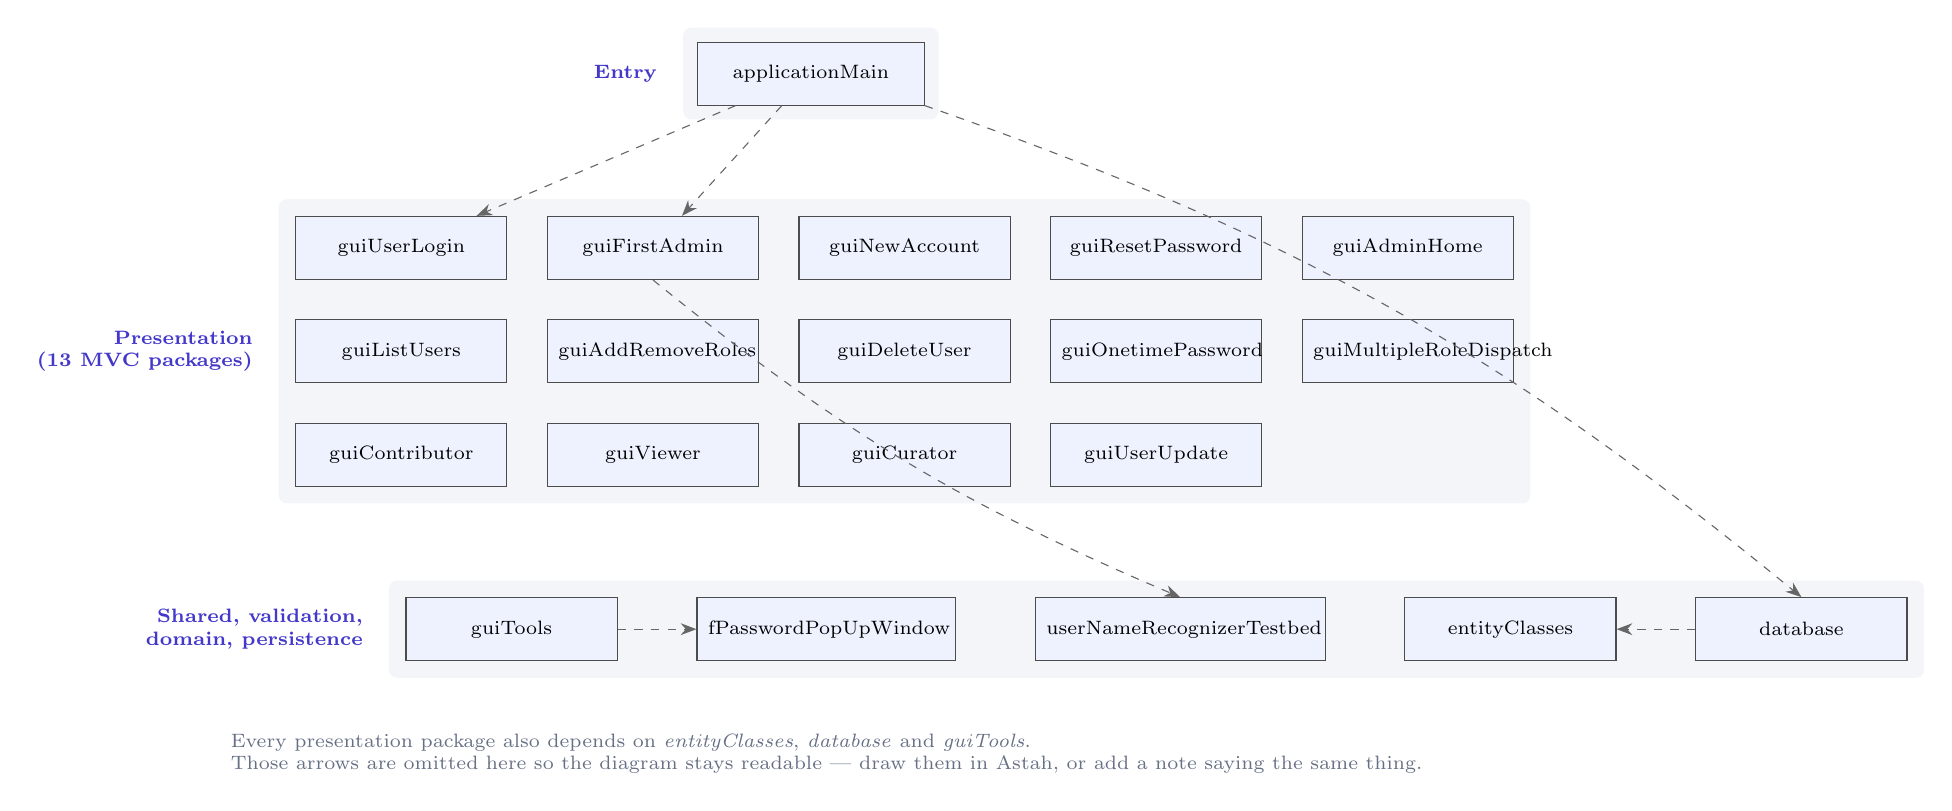
\begin{tikzpicture}[node distance=5mm]

  % --- Entry layer -----------------------------------------------------
  \node[pkg=26mm] (main) {applicationMain};

  % --- Presentation layer ----------------------------------------------
  \node[pkg=24mm, below=14mm of main, xshift=-52mm] (login)   {guiUserLogin};
  \node[pkg=24mm, right=of login]                   (first)   {guiFirstAdmin};
  \node[pkg=24mm, right=of first]                   (newacc)  {guiNewAccount};
  \node[pkg=24mm, right=of newacc]                  (reset)   {guiResetPassword};
  \node[pkg=24mm, right=of reset]                   (adminh)  {guiAdminHome};

  \node[pkg=24mm, below=of login]   (listu)   {guiListUsers};
  \node[pkg=24mm, right=of listu]   (roles)   {guiAddRemoveRoles};
  \node[pkg=24mm, right=of roles]   (del)     {guiDeleteUser};
  \node[pkg=24mm, right=of del]     (otp)     {guiOnetimePassword};
  \node[pkg=24mm, right=of otp]     (disp)    {guiMultipleRoleDispatch};

  \node[pkg=24mm, below=of listu]   (contrib) {guiContributor};
  \node[pkg=24mm, right=of contrib] (viewer)  {guiViewer};
  \node[pkg=24mm, right=of viewer]  (curator) {guiCurator};
  \node[pkg=24mm, right=of curator] (update)  {guiUserUpdate};

  % --- Shared, validation, domain, persistence -------------------------
  \node[pkg=24mm, below=14mm of contrib, xshift=14mm] (tools) {guiTools};
  \node[pkg=30mm, right=10mm of tools] (pwd)   {fPasswordPopUpWindow};
  \node[pkg=34mm, right=10mm of pwd]   (unr)   {userNameRecognizerTestbed};
  \node[pkg=24mm, right=10mm of unr]   (ent)   {entityClasses};
  \node[pkg=24mm, right=10mm of ent]   (db)    {database};

  % --- Layer bands ------------------------------------------------------
  \begin{scope}[on background layer]
    \node[band, fit=(main), inner sep=5pt] (b1) {};
    \node[band, fit=(login)(adminh)(contrib)(update), inner sep=6pt] (b2) {};
    \node[band, fit=(tools)(db), inner sep=6pt] (b3) {};
  \end{scope}

  \node[font=\scriptsize\bfseries, color=accent, left=2mm of b1] {Entry};
  \node[font=\scriptsize\bfseries, color=accent, left=2mm of b2, align=right]
       {Presentation\\(13 MVC packages)};
  \node[font=\scriptsize\bfseries, color=accent, left=2mm of b3, align=right]
       {Shared, validation,\\domain, persistence};

  % --- Dependencies -----------------------------------------------------
  \draw[uses] (main) -- (login);
  \draw[uses] (main) -- (first);
  \draw[uses] (main.south east) to[bend left=10] (db.north);
  \draw[uses] (tools) -- (pwd);
  \draw[uses] (first.south) to[bend right=8] (unr.north);
  \draw[uses] (db) -- (ent);

  \node[font=\scriptsize, color=muted, align=left, below=8mm of tools, xshift=40mm]
       {Every presentation package also depends on
        \textit{entityClasses}, \textit{database} and \textit{guiTools}.\\
        Those arrows are omitted here so the diagram stays readable ---
        draw them in Astah, or add a note saying the same thing.};

\end{tikzpicture}
\caption{System architecture, grouped by layer}
\end{figure}

\newpage
%=======================================================================
%  2. NAVIGATION DIAGRAM
%=======================================================================
\section*{2. Navigation between pages}

Every page also has a \textit{Logout} edge back to Login; those are omitted so the
structural edges stay visible.

\begin{figure}[H]
\centering
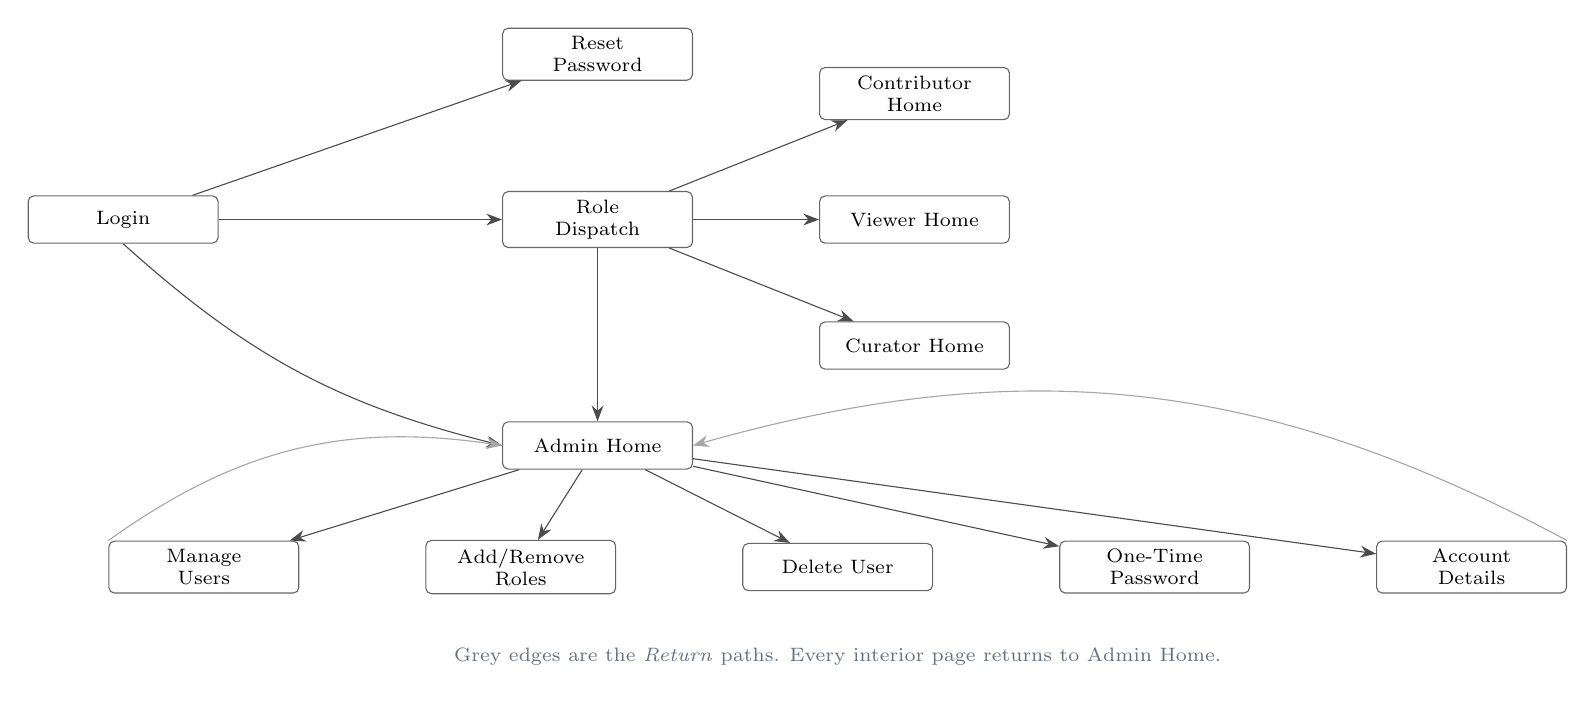
\begin{tikzpicture}[node distance=9mm and 16mm]

  \node[page=22mm] (login) {Login};
  \node[page=22mm, right=36mm of login] (disp) {Role\\Dispatch};
  \node[page=22mm, below=22mm of disp]  (admin) {Admin Home};
  \node[page=22mm, above=14mm of disp]  (reset) {Reset\\Password};

  \node[page=22mm, right=of disp, yshift=16mm] (contrib) {Contributor\\Home};
  \node[page=22mm, right=of disp]              (viewer)  {Viewer Home};
  \node[page=22mm, right=of disp, yshift=-16mm](curator) {Curator Home};

  \node[page=22mm, below=of admin, xshift=-50mm] (listu) {Manage\\Users};
  \node[page=22mm, right=of listu]  (roles)  {Add/Remove\\Roles};
  \node[page=22mm, right=of roles]  (del)    {Delete User};
  \node[page=22mm, right=of del]    (otp)    {One-Time\\Password};
  \node[page=22mm, right=of otp]    (update) {Account\\Details};

  \draw[calls] (login) -- (disp);
  \draw[calls] (login) -- (reset);
  \draw[calls] (login.south) to[bend right=14] (admin.west);

  \draw[calls] (disp) -- (admin);
  \draw[calls] (disp) -- (contrib);
  \draw[calls] (disp) -- (viewer);
  \draw[calls] (disp) -- (curator);

  \draw[calls] (admin) -- (listu);
  \draw[calls] (admin) -- (roles);
  \draw[calls] (admin) -- (del);
  \draw[calls] (admin) -- (otp);
  \draw[calls] (admin) -- (update);

  \draw[calls, draw=black!35] (listu.north west)  to[bend left=22]  (admin.west);
  \draw[calls, draw=black!35] (update.north east) to[bend right=22] (admin.east);

  \node[font=\scriptsize, color=muted, below=6mm of del, align=center]
       {Grey edges are the \textit{Return} paths. Every interior page returns to Admin Home.};

\end{tikzpicture}
\caption{Page navigation. There is no router --- each page calls the next page directly}
\end{figure}

\newpage
%=======================================================================
%  3. CLASS DIAGRAM -- DOMAIN AND PERSISTENCE
%=======================================================================
\section*{3. Class diagram --- domain and persistence}

\begin{figure}[H]
\centering
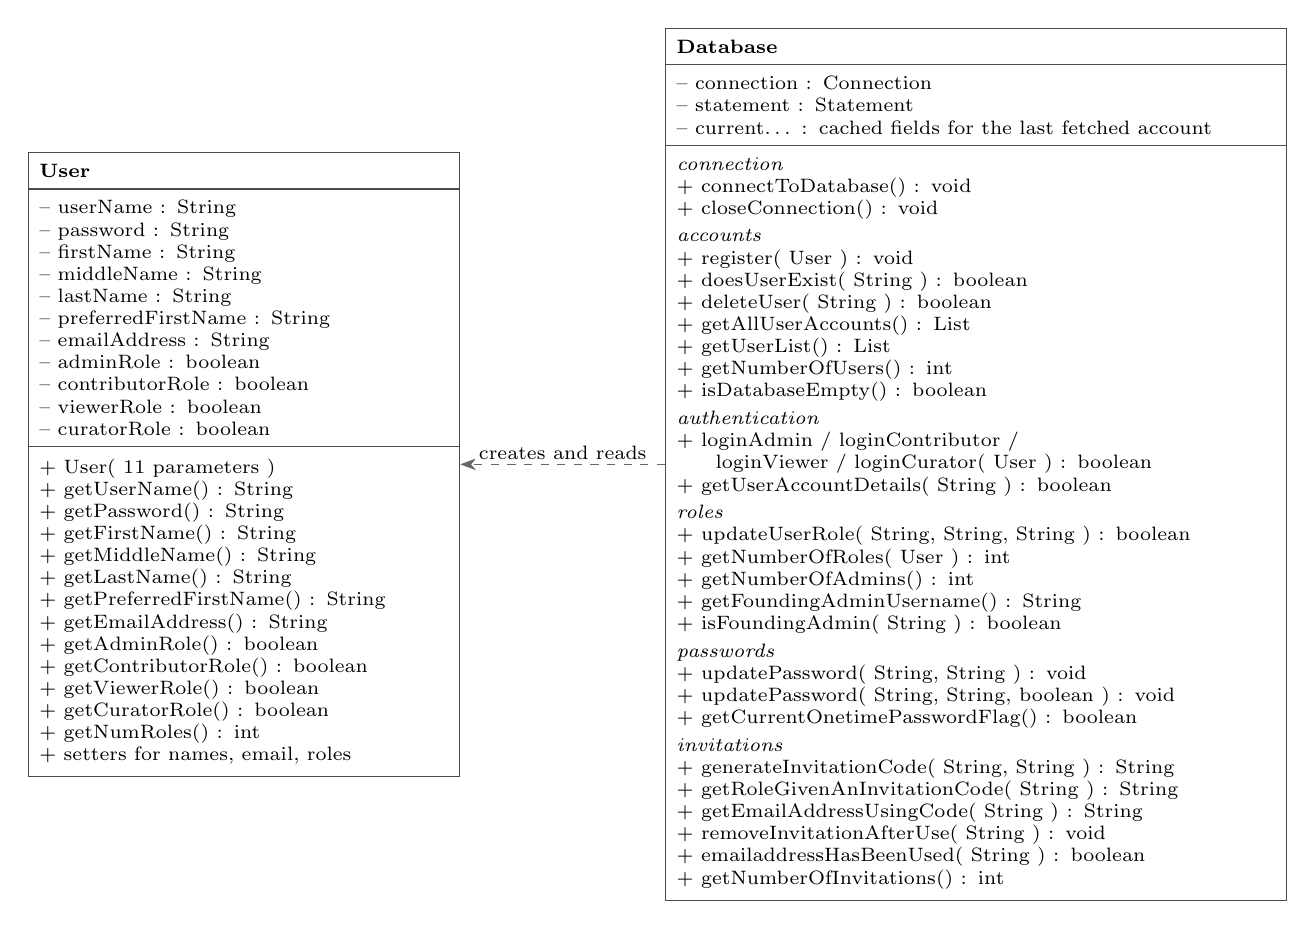
\begin{tikzpicture}

\node[umlclass=52mm] (user) {
  \textbf{User}
  \nodepart{two}
    -- userName : String\\
    -- password : String\\
    -- firstName : String\\
    -- middleName : String\\
    -- lastName : String\\
    -- preferredFirstName : String\\
    -- emailAddress : String\\
    -- adminRole : boolean\\
    -- contributorRole : boolean\\
    -- viewerRole : boolean\\
    -- curatorRole : boolean
  \nodepart{three}
    + User( 11 parameters )\\
    + getUserName() : String\\
    + getPassword() : String\\
    + getFirstName() : String\\
    + getMiddleName() : String\\
    + getLastName() : String\\
    + getPreferredFirstName() : String\\
    + getEmailAddress() : String\\
    + getAdminRole() : boolean\\
    + getContributorRole() : boolean\\
    + getViewerRole() : boolean\\
    + getCuratorRole() : boolean\\
    + getNumRoles() : int\\
    + setters for names, email, roles
};

\node[umlclass=76mm, right=26mm of user] (db) {
  \textbf{Database}
  \nodepart{two}
    -- connection : Connection\\
    -- statement : Statement\\
    -- current\dots\ : cached fields for the last fetched account
  \nodepart{three}
    \textit{connection}\\
    + connectToDatabase() : void\\
    + closeConnection() : void\\[2pt]
    \textit{accounts}\\
    + register( User ) : void\\
    + doesUserExist( String ) : boolean\\
    + deleteUser( String ) : boolean\\
    + getAllUserAccounts() : List\\
    + getUserList() : List\\
    + getNumberOfUsers() : int\\
    + isDatabaseEmpty() : boolean\\[2pt]
    \textit{authentication}\\
    + loginAdmin / loginContributor /\\
    \hspace*{4mm} loginViewer / loginCurator( User ) : boolean\\
    + getUserAccountDetails( String ) : boolean\\[2pt]
    \textit{roles}\\
    + updateUserRole( String, String, String ) : boolean\\
    + getNumberOfRoles( User ) : int\\
    + getNumberOfAdmins() : int\\
    + getFoundingAdminUsername() : String\\
    + isFoundingAdmin( String ) : boolean\\[2pt]
    \textit{passwords}\\
    + updatePassword( String, String ) : void\\
    + updatePassword( String, String, boolean ) : void\\
    + getCurrentOnetimePasswordFlag() : boolean\\[2pt]
    \textit{invitations}\\
    + generateInvitationCode( String, String ) : String\\
    + getRoleGivenAnInvitationCode( String ) : String\\
    + getEmailAddressUsingCode( String ) : String\\
    + removeInvitationAfterUse( String ) : void\\
    + emailaddressHasBeenUsed( String ) : boolean\\
    + getNumberOfInvitations() : int
};

\draw[uses] (db.west) -- node[lbl, midway, above]{creates and reads} (user.east);

\end{tikzpicture}
\caption{The only domain type, and the single class that owns all persistence}
\end{figure}

\newpage
%=======================================================================
%  4. CLASS DIAGRAM -- THE MVC PAGE PATTERN
%=======================================================================
\section*{4. Class diagram --- the MVC page pattern}

All thirteen page packages share this shape. \texttt{guiListUsers} is shown as the concrete
example because it is the one whose Model actually holds logic.

\begin{figure}[H]
\centering
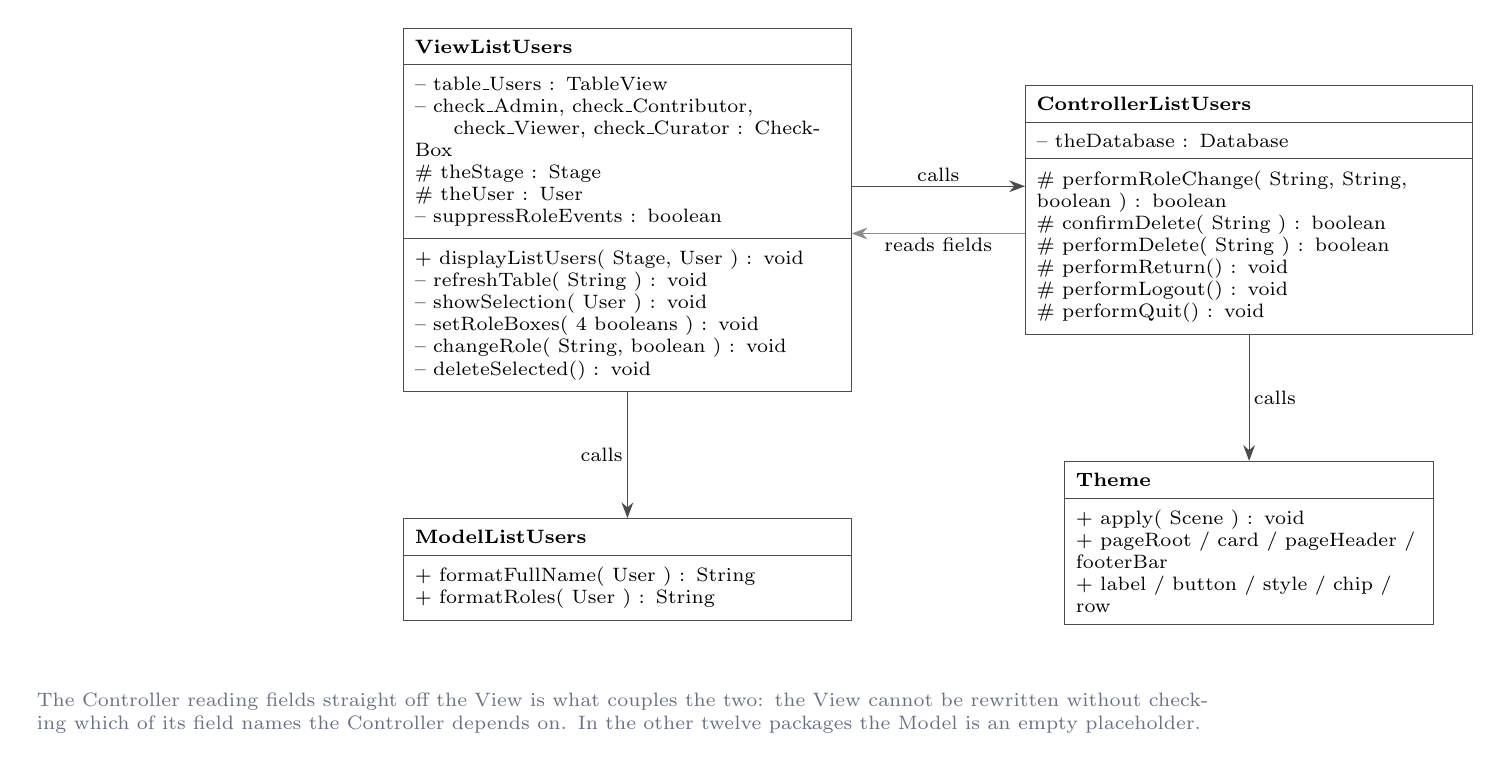
\begin{tikzpicture}

\node[umlclass=54mm] (view) {
  \textbf{ViewListUsers}
  \nodepart{two}
    -- table\_Users : TableView\\
    -- check\_Admin, check\_Contributor,\\
    \hspace*{4mm} check\_Viewer, check\_Curator : CheckBox\\
    \# theStage : Stage\\
    \# theUser : User\\
    -- suppressRoleEvents : boolean
  \nodepart{three}
    + displayListUsers( Stage, User ) : void\\
    -- refreshTable( String ) : void\\
    -- showSelection( User ) : void\\
    -- setRoleBoxes( 4 booleans ) : void\\
    -- changeRole( String, boolean ) : void\\
    -- deleteSelected() : void
};

\node[umlclass=54mm, right=22mm of view] (ctrl) {
  \textbf{ControllerListUsers}
  \nodepart{two}
    -- theDatabase : Database
  \nodepart{three}
    \# performRoleChange( String, String, boolean ) : boolean\\
    \# confirmDelete( String ) : boolean\\
    \# performDelete( String ) : boolean\\
    \# performReturn() : void\\
    \# performLogout() : void\\
    \# performQuit() : void
};

\node[umlclasstwo=54mm, below=16mm of view] (model) {
  \textbf{ModelListUsers}
  \nodepart{two}
    + formatFullName( User ) : String\\
    + formatRoles( User ) : String
};

\node[umlclasstwo=44mm, below=16mm of ctrl] (theme) {
  \textbf{Theme}
  \nodepart{two}
    + apply( Scene ) : void\\
    + pageRoot / card / pageHeader / footerBar\\
    + label / button / style / chip / row
};

\draw[calls] ($(view.east)+(0,3mm)$) -- node[lbl, midway, above]{calls}
             ($(ctrl.west)+(0,3mm)$);
\draw[calls, draw=black!45] ($(ctrl.west)+(0,-3mm)$) --
             node[lbl, midway, below]{reads fields} ($(view.east)+(0,-3mm)$);
\draw[calls] (view) -- node[lbl, midway, left]{calls} (model);
\draw[calls] (ctrl) -- node[lbl, midway, right]{calls} (theme);

\node[font=\scriptsize, color=muted, below=8mm of model, align=left, text width=150mm]
  {The Controller reading fields straight off the View is what couples the two: the View
   cannot be rewritten without checking which of its field names the Controller depends on.
   In the other twelve packages the Model is an empty placeholder.};

\end{tikzpicture}
\caption{The Model--View--Controller shape every page package follows}
\end{figure}

\newpage
%=======================================================================
%  5. CLASS DIAGRAM -- SHARED SERVICES
%=======================================================================
\section*{5. Class diagram --- shared services and validation}

\begin{figure}[H]
\centering
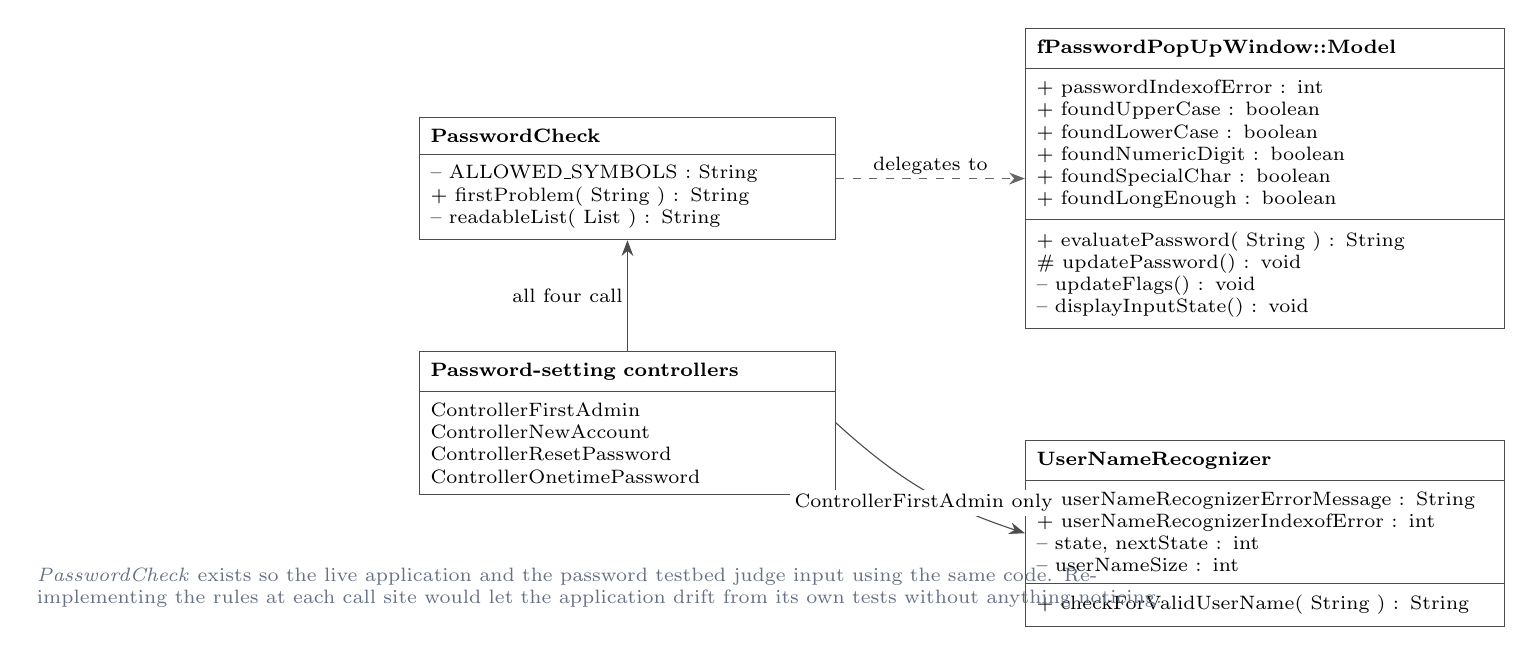
\begin{tikzpicture}

\node[umlclasstwo=50mm] (pwc) {
  \textbf{PasswordCheck}
  \nodepart{two}
    -- ALLOWED\_SYMBOLS : String\\
    + firstProblem( String ) : String\\
    -- readableList( List ) : String
};

\node[umlclass=58mm, right=24mm of pwc] (pwm) {
  \textbf{fPasswordPopUpWindow::Model}
  \nodepart{two}
    + passwordIndexofError : int\\
    + foundUpperCase : boolean\\
    + foundLowerCase : boolean\\
    + foundNumericDigit : boolean\\
    + foundSpecialChar : boolean\\
    + foundLongEnough : boolean
  \nodepart{three}
    + evaluatePassword( String ) : String\\
    \# updatePassword() : void\\
    -- updateFlags() : void\\
    -- displayInputState() : void
};

\node[umlclass=58mm, below=14mm of pwm] (unr) {
  \textbf{UserNameRecognizer}
  \nodepart{two}
    + userNameRecognizerErrorMessage : String\\
    + userNameRecognizerIndexofError : int\\
    -- state, nextState : int\\
    -- userNameSize : int
  \nodepart{three}
    + checkForValidUserName( String ) : String
};

\node[umlclasstwo=50mm, below=14mm of pwc] (callers) {
  \textbf{Password-setting controllers}
  \nodepart{two}
    ControllerFirstAdmin\\
    ControllerNewAccount\\
    ControllerResetPassword\\
    ControllerOnetimePassword
};

\draw[uses] (pwc) -- node[lbl, midway, above]{delegates to} (pwm);
\draw[calls] (callers) -- node[lbl, midway, left]{all four call} (pwc);
\draw[calls] (callers.east) to[bend right=12]
      node[lbl, midway, below]{ControllerFirstAdmin only} (unr.west);

\node[font=\scriptsize, color=muted, below=8mm of callers, align=left, text width=150mm]
  {\textit{PasswordCheck} exists so the live application and the password testbed judge
   input using the same code. Re-implementing the rules at each call site would let the
   application drift from its own tests without anything noticing.};

\end{tikzpicture}
\caption{Validation reached through a single facade}
\end{figure}

\newpage
%=======================================================================
%  6. STATE MACHINE -- USERNAME RECOGNIZER
%=======================================================================
\section*{6. State machine --- username recognizer}

\begin{figure}[H]
\centering
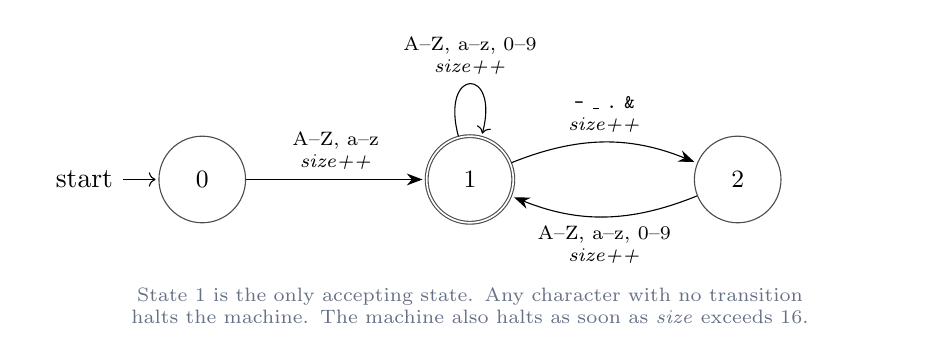
\begin{tikzpicture}[shorten >=1pt, node distance=34mm, on grid, auto,
                    every state/.style={draw=black!70, fill=white,
                                        minimum size=11mm, font=\small}]

  \node[state, initial, initial text={start}] (s0) {0};
  \node[state, accepting, right=of s0]        (s1) {1};
  \node[state, right=of s1]                   (s2) {2};

  \path[-{Stealth[length=2mm]}]
    (s0) edge              node[font=\scriptsize, align=center]
                                {A--Z, a--z\\\textit{size++}} (s1)
    (s1) edge[loop above]  node[font=\scriptsize, align=center]
                                {A--Z, a--z, 0--9\\\textit{size++}} ()
    (s1) edge[bend left=22] node[font=\scriptsize, align=center]
                                {\texttt{-}\ \texttt{\_}\ \texttt{.}\ \texttt{\&}\\\textit{size++}} (s2)
    (s2) edge[bend left=22] node[font=\scriptsize, align=center]
                                {A--Z, a--z, 0--9\\\textit{size++}} (s1);

  \node[font=\scriptsize, color=muted, below=16mm of s1, align=center, text width=110mm]
    {State 1 is the only accepting state. Any character with no transition halts the
     machine. The machine also halts as soon as \textit{size} exceeds 16.};

\end{tikzpicture}
\caption{Username recognizer. Three states, one of them accepting}
\end{figure}

\textbf{Verdict when the machine halts}

\begin{center}
\begin{tabular}{@{}cll@{}}
\hline
\textbf{Halt state} & \textbf{Condition} & \textbf{Result}\\
\hline
0 & ---                       & Rejected: must start with a letter\\
1 & size $<$ 4                & Rejected: at least 4 characters\\
1 & size $>$ 16               & Rejected: no more than 16 characters\\
1 & input not fully consumed  & Rejected: contains a character that is not allowed\\
1 & 4--16, fully consumed     & \textbf{Accepted}\\
2 & ---                       & Rejected: a separator must be followed by a letter or digit\\
\hline
\end{tabular}
\end{center}

\newpage
%=======================================================================
%  7. STATE MACHINE -- PASSWORD RECOGNIZER
%=======================================================================
\section*{7. State machine --- password recognizer}

\begin{figure}[H]
\centering
\begin{tikzpicture}[shorten >=1pt, node distance=40mm, on grid, auto,
                    every state/.style={draw=black!70, fill=white,
                                        minimum size=13mm, font=\scriptsize,
                                        align=center}]

  \node[state, initial, initial text={start}] (scan) {Scanning};
  \node[state, right=46mm of scan]            (eval) {Evaluate};
  \node[state, accepting, right=42mm of eval] (ok)   {Accepted};
  \node[state, below=26mm of eval]            (bad)  {Rejected};
  \node[state, below=26mm of scan]            (inv)  {Invalid\\character};

  \path[-{Stealth[length=2mm]}]
    (scan) edge[loop above] node[font=\scriptsize, align=center]
              {A--Z / foundUpperCase\\a--z / foundLowerCase} ()
    (scan) edge[loop below, looseness=6] node[font=\scriptsize, align=center, yshift=-2mm]
              {0--9 / foundNumericDigit\\symbol / foundSpecialChar\\index $\geq$ 7 / foundLongEnough} ()
    (scan) edge node[font=\scriptsize]{end of input} (eval)
    (scan) edge node[font=\scriptsize, align=center, swap]
              {character in no\\accepted class} (inv)
    (eval) edge node[font=\scriptsize, align=center]{all five\\flags set} (ok)
    (eval) edge node[font=\scriptsize, align=center, swap]{any flag\\not set} (bad);

\end{tikzpicture}
\caption{Password recognizer. One scanning state that sets a flag per requirement}
\end{figure}

\textbf{The five requirements}, all of which must hold: at least one upper case letter, at
least one lower case letter, at least one digit, at least one accepted symbol, and a length
of at least eight characters.

An empty password is rejected before scanning begins. \textbf{A space is not an accepted
character}, so a passphrase halts the machine at the space and is reported as containing a
character that is not allowed, rather than as a weak password.

\newpage
%=======================================================================
%  8. ER DIAGRAM
%=======================================================================
\section*{8. Data model}

\begin{figure}[H]
\centering
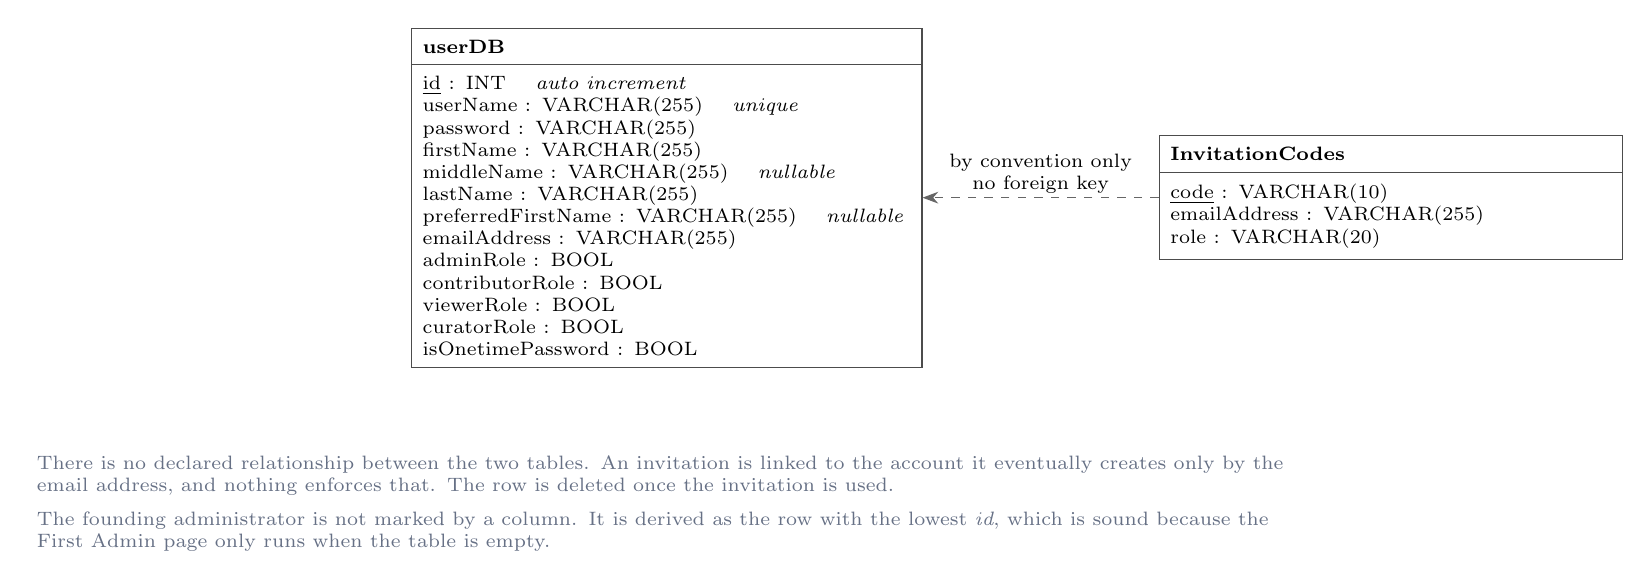
\begin{tikzpicture}

\node[umlclasstwo=62mm] (users) {
  \textbf{userDB}
  \nodepart{two}
    \underline{id} : INT \quad\textit{auto increment}\\
    userName : VARCHAR(255) \quad\textit{unique}\\
    password : VARCHAR(255)\\
    firstName : VARCHAR(255)\\
    middleName : VARCHAR(255) \quad\textit{nullable}\\
    lastName : VARCHAR(255)\\
    preferredFirstName : VARCHAR(255) \quad\textit{nullable}\\
    emailAddress : VARCHAR(255)\\
    adminRole : BOOL\\
    contributorRole : BOOL\\
    viewerRole : BOOL\\
    curatorRole : BOOL\\
    isOnetimePassword : BOOL
};

\node[umlclasstwo=56mm, right=30mm of users] (inv) {
  \textbf{InvitationCodes}
  \nodepart{two}
    \underline{code} : VARCHAR(10)\\
    emailAddress : VARCHAR(255)\\
    role : VARCHAR(20)
};

\draw[uses] (inv.west) -- node[lbl, midway, above, align=center]
     {by convention only\\no foreign key} (users.east);

\node[font=\scriptsize, color=muted, below=10mm of users, align=left, text width=160mm]
  {There is no declared relationship between the two tables. An invitation is linked to the
   account it eventually creates only by the email address, and nothing enforces that. The
   row is deleted once the invitation is used.\\[4pt]
   The founding administrator is not marked by a column. It is derived as the row with the
   lowest \textit{id}, which is sound because the First Admin page only runs when the table
   is empty.};

\end{tikzpicture}
\caption{Two tables, no foreign key between them}
\end{figure}

\newpage
%=======================================================================
%  9. SEQUENCE -- LOGIN
%=======================================================================
\section*{9. Sequence --- logging in}

\begin{figure}[H]
\centering
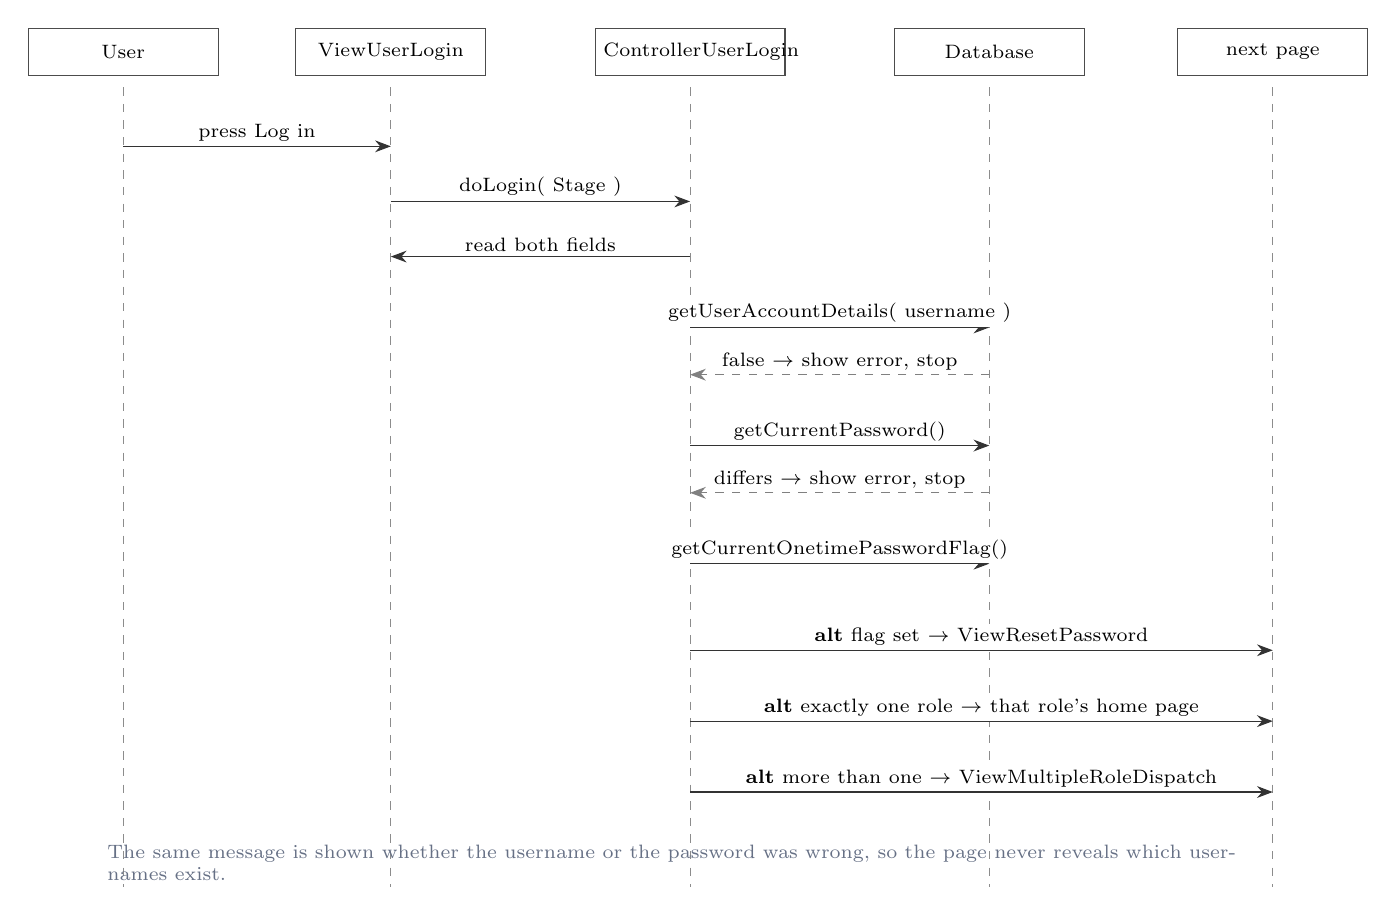
\begin{tikzpicture}[font=\scriptsize]

  \lifeline{0}{a}{User}{-10.6}
  \lifeline{3.4}{b}{ViewUserLogin}{-10.6}
  \lifeline{7.2}{c}{ControllerUserLogin}{-10.6}
  \lifeline{11.0}{d}{Database}{-10.6}
  \lifeline{14.6}{e}{next page}{-10.6}

  \msgarrow{0}{3.4}{-1.2}{press Log in}
  \msgarrow{3.4}{7.2}{-1.9}{doLogin( Stage )}
  \draw[msg] (7.2,-2.6) -- (3.4,-2.6) node[lbl, midway, above]{read both fields};

  \msgarrow{7.2}{11.0}{-3.5}{getUserAccountDetails( username )}
  \draw[ret] (11.0,-4.1) -- (7.2,-4.1) node[lbl, midway, above]{false $\rightarrow$ show error, stop};

  \msgarrow{7.2}{11.0}{-5.0}{getCurrentPassword()}
  \draw[ret] (11.0,-5.6) -- (7.2,-5.6) node[lbl, midway, above]{differs $\rightarrow$ show error, stop};

  \msgarrow{7.2}{11.0}{-6.5}{getCurrentOnetimePasswordFlag()}

  \draw[msg] (7.2,-7.6) -- (14.6,-7.6)
        node[lbl, midway, above]{\textbf{alt} flag set $\rightarrow$ ViewResetPassword};
  \draw[msg] (7.2,-8.5) -- (14.6,-8.5)
        node[lbl, midway, above]{\textbf{alt} exactly one role $\rightarrow$ that role's home page};
  \draw[msg] (7.2,-9.4) -- (14.6,-9.4)
        node[lbl, midway, above]{\textbf{alt} more than one $\rightarrow$ ViewMultipleRoleDispatch};

  \node[font=\scriptsize, color=muted, align=left, text width=150mm] at (7.3,-10.3)
    {The same message is shown whether the username or the password was wrong, so the page
     never reveals which usernames exist.};

\end{tikzpicture}
\caption{Logging in, including the one-time-password branch}
\end{figure}

\newpage
%=======================================================================
%  10. SEQUENCE -- FIRST ADMINISTRATOR
%=======================================================================
\section*{10. Sequence --- setting up the first administrator}

\begin{figure}[H]
\centering
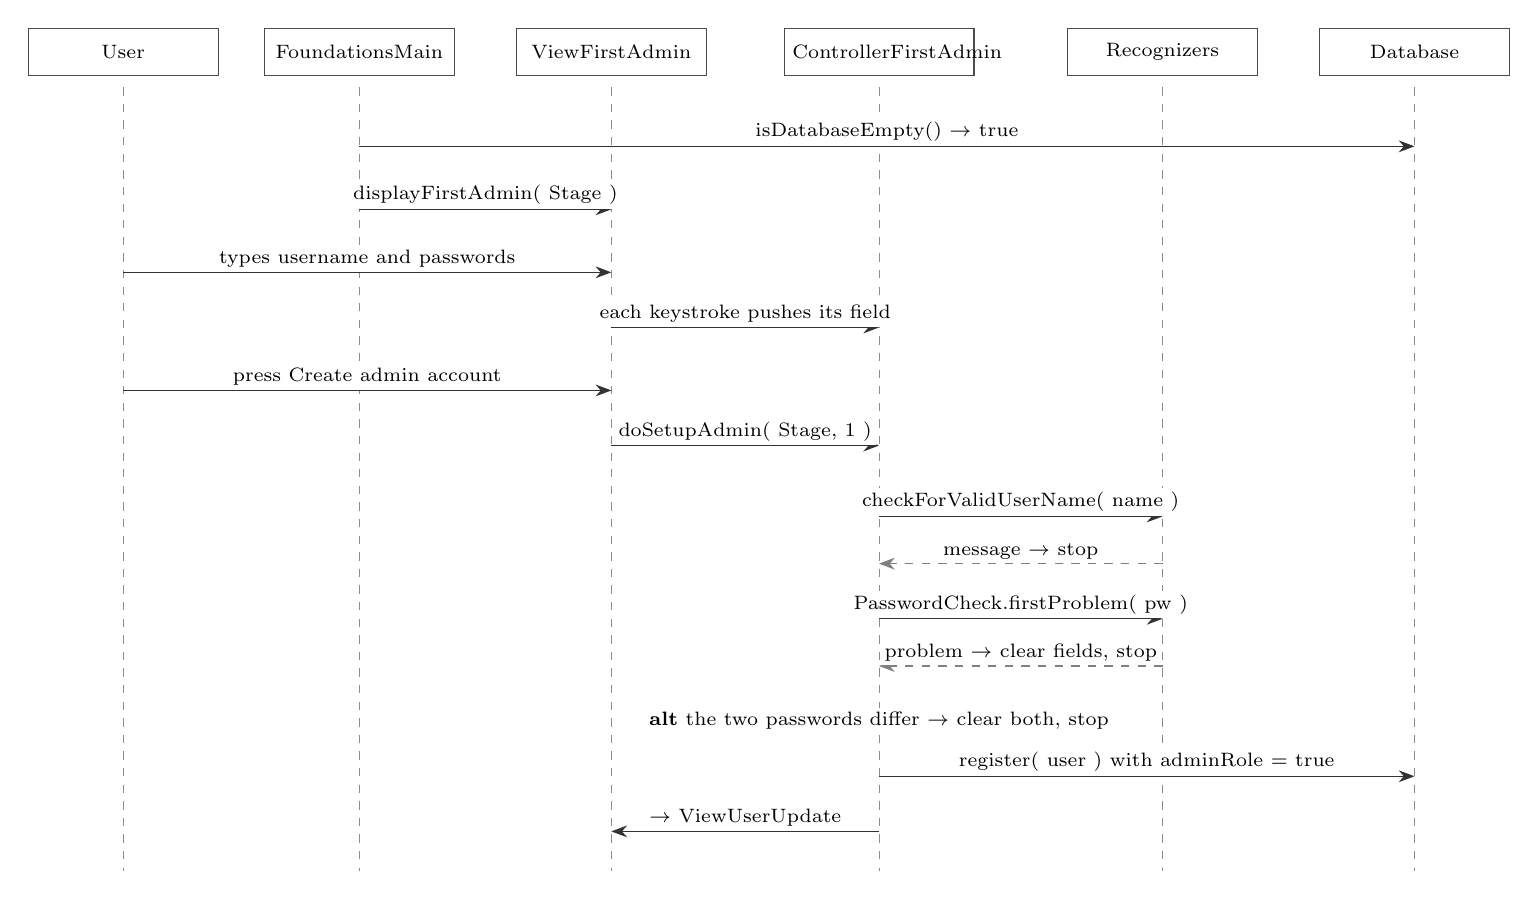
\begin{tikzpicture}[font=\scriptsize]

  \lifeline{0}{a}{User}{-10.4}
  \lifeline{3.0}{b}{FoundationsMain}{-10.4}
  \lifeline{6.2}{c}{ViewFirstAdmin}{-10.4}
  \lifeline{9.6}{d}{ControllerFirstAdmin}{-10.4}
  \lifeline{13.2}{e}{Recognizers}{-10.4}
  \lifeline{16.4}{f}{Database}{-10.4}

  \msgarrow{3.0}{16.4}{-1.2}{isDatabaseEmpty() $\rightarrow$ true}
  \msgarrow{3.0}{6.2}{-2.0}{displayFirstAdmin( Stage )}
  \msgarrow{0}{6.2}{-2.8}{types username and passwords}
  \draw[msg] (6.2,-3.5) -- (9.6,-3.5)
        node[lbl, midway, above]{each keystroke pushes its field};
  \msgarrow{0}{6.2}{-4.3}{press Create admin account}
  \msgarrow{6.2}{9.6}{-5.0}{doSetupAdmin( Stage, 1 )}

  \msgarrow{9.6}{13.2}{-5.9}{checkForValidUserName( name )}
  \draw[ret] (13.2,-6.5) -- (9.6,-6.5) node[lbl, midway, above]{message $\rightarrow$ stop};

  \msgarrow{9.6}{13.2}{-7.2}{PasswordCheck.firstProblem( pw )}
  \draw[ret] (13.2,-7.8) -- (9.6,-7.8) node[lbl, midway, above]{problem $\rightarrow$ clear fields, stop};

  \node[lbl, align=left] at (9.6,-8.5) {\textbf{alt} the two passwords differ $\rightarrow$ clear both, stop};

  \msgarrow{9.6}{16.4}{-9.2}{register( user ) with adminRole = true}
  \msgarrow{9.6}{6.2}{-9.9}{$\rightarrow$ ViewUserUpdate}

\end{tikzpicture}
\caption{First administrator setup. Both recognizers run before the passwords are compared}
\end{figure}

\newpage
%=======================================================================
%  11. SEQUENCE -- INVITATION TO ACCOUNT
%=======================================================================
\section*{11. Sequence --- invitation to account creation}

\begin{figure}[H]
\centering
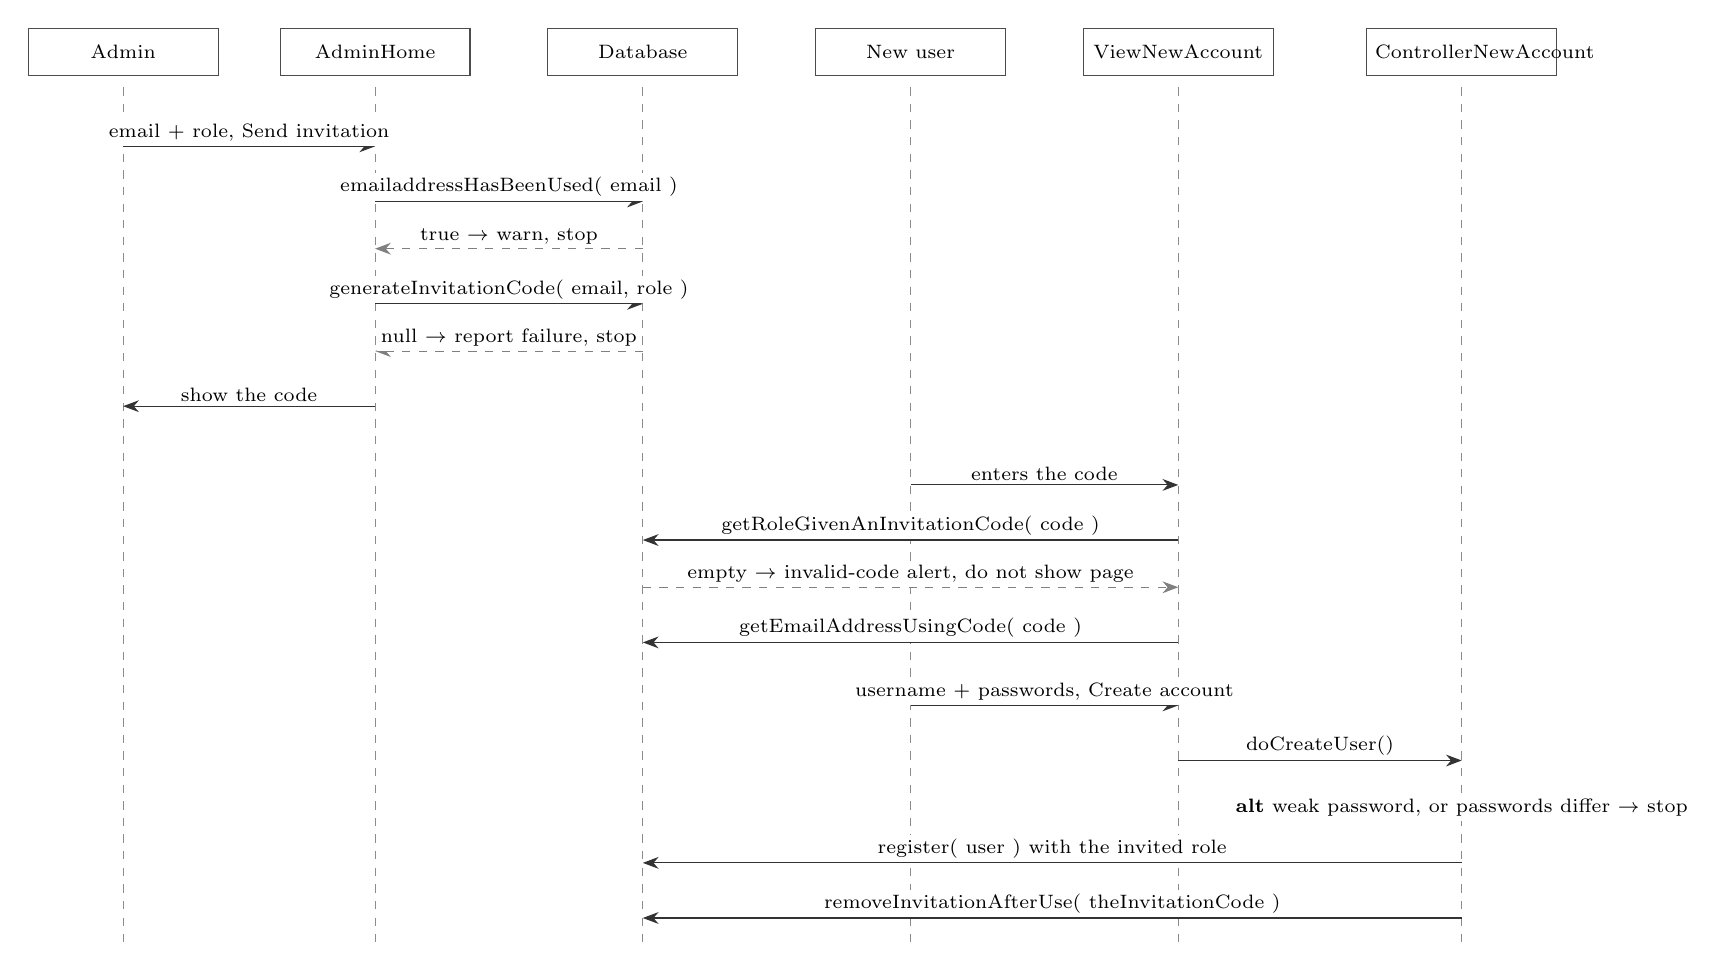
\begin{tikzpicture}[font=\scriptsize]

  \lifeline{0}{a}{Admin}{-11.4}
  \lifeline{3.2}{b}{AdminHome}{-11.4}
  \lifeline{6.6}{c}{Database}{-11.4}
  \lifeline{10.0}{d}{New user}{-11.4}
  \lifeline{13.4}{e}{ViewNewAccount}{-11.4}
  \lifeline{17.0}{f}{ControllerNewAccount}{-11.4}

  \msgarrow{0}{3.2}{-1.2}{email + role, Send invitation}
  \msgarrow{3.2}{6.6}{-1.9}{emailaddressHasBeenUsed( email )}
  \draw[ret] (6.6,-2.5) -- (3.2,-2.5) node[lbl, midway, above]{true $\rightarrow$ warn, stop};

  \msgarrow{3.2}{6.6}{-3.2}{generateInvitationCode( email, role )}
  \draw[ret] (6.6,-3.8) -- (3.2,-3.8) node[lbl, midway, above]{null $\rightarrow$ report failure, stop};
  \draw[msg] (3.2,-4.5) -- (0,-4.5) node[lbl, midway, above]{show the code};

  \msgarrow{10.0}{13.4}{-5.5}{enters the code}
  \msgarrow{13.4}{6.6}{-6.2}{getRoleGivenAnInvitationCode( code )}
  \draw[ret] (6.6,-6.8) -- (13.4,-6.8) node[lbl, midway, above]{empty $\rightarrow$ invalid-code alert, do not show page};
  \msgarrow{13.4}{6.6}{-7.5}{getEmailAddressUsingCode( code )}

  \msgarrow{10.0}{13.4}{-8.3}{username + passwords, Create account}
  \msgarrow{13.4}{17.0}{-9.0}{doCreateUser()}
  \node[lbl, align=left] at (17.0,-9.6) {\textbf{alt} weak password, or passwords differ $\rightarrow$ stop};

  \msgarrow{17.0}{6.6}{-10.3}{register( user ) with the invited role}
  \msgarrow{17.0}{6.6}{-11.0}{removeInvitationAfterUse( theInvitationCode )}

\end{tikzpicture}
\caption{Invitation through to account creation. The final message is what consumes the code}
\end{figure}

\newpage
%=======================================================================
%  12. SEQUENCE -- ROLE CHANGE
%=======================================================================
\section*{12. Sequence --- changing a user's roles}

\begin{figure}[H]
\centering
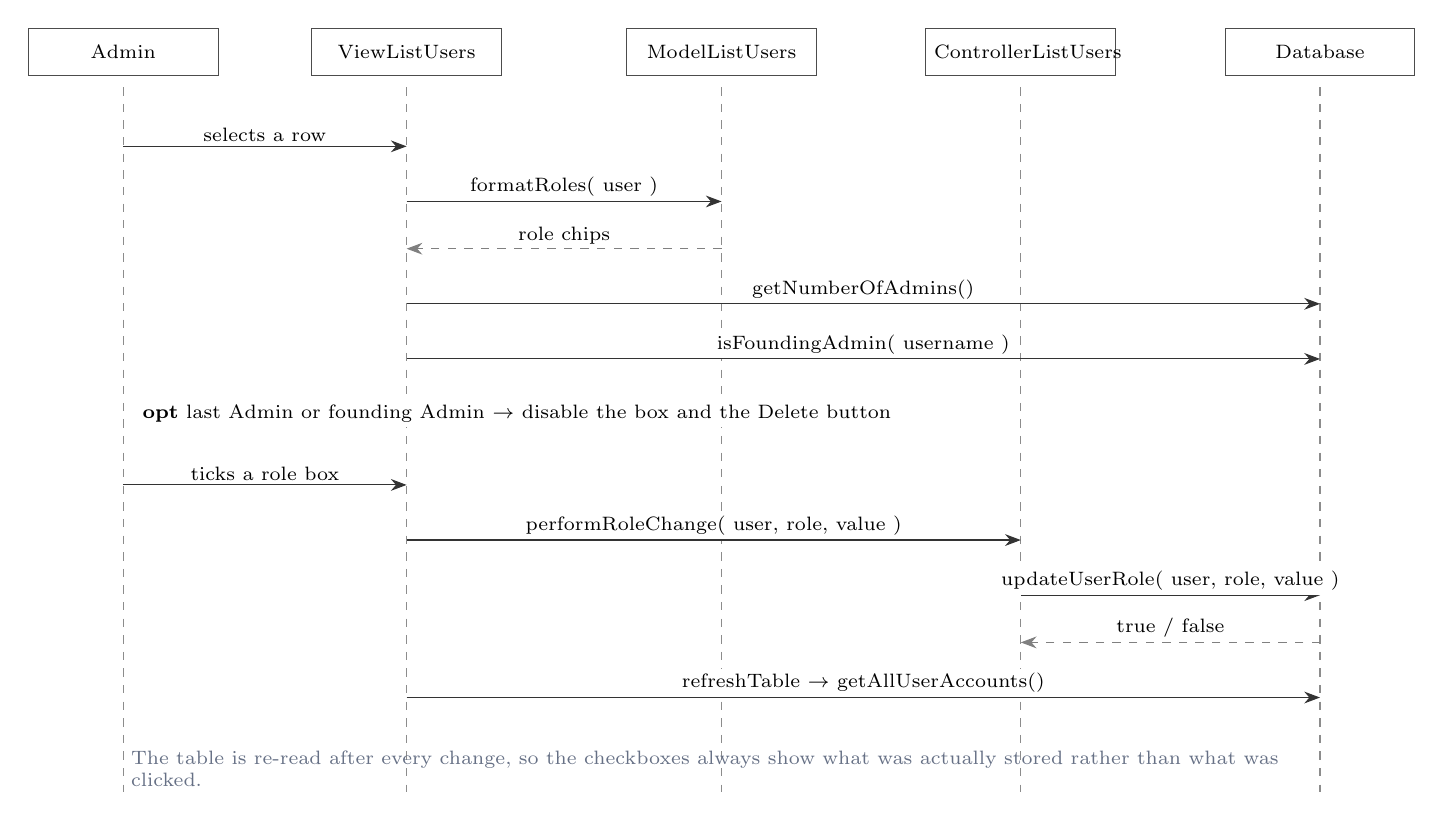
\begin{tikzpicture}[font=\scriptsize]

  \lifeline{0}{a}{Admin}{-9.4}
  \lifeline{3.6}{b}{ViewListUsers}{-9.4}
  \lifeline{7.6}{c}{ModelListUsers}{-9.4}
  \lifeline{11.4}{d}{ControllerListUsers}{-9.4}
  \lifeline{15.2}{e}{Database}{-9.4}

  \msgarrow{0}{3.6}{-1.2}{selects a row}
  \msgarrow{3.6}{7.6}{-1.9}{formatRoles( user )}
  \draw[ret] (7.6,-2.5) -- (3.6,-2.5) node[lbl, midway, above]{role chips};

  \msgarrow{3.6}{15.2}{-3.2}{getNumberOfAdmins()}
  \msgarrow{3.6}{15.2}{-3.9}{isFoundingAdmin( username )}
  \node[lbl, align=left] at (5.0,-4.6)
       {\textbf{opt} last Admin or founding Admin $\rightarrow$ disable the box and the Delete button};

  \msgarrow{0}{3.6}{-5.5}{ticks a role box}
  \msgarrow{3.6}{11.4}{-6.2}{performRoleChange( user, role, value )}
  \msgarrow{11.4}{15.2}{-6.9}{updateUserRole( user, role, value )}
  \draw[ret] (15.2,-7.5) -- (11.4,-7.5) node[lbl, midway, above]{true / false};

  \msgarrow{3.6}{15.2}{-8.2}{refreshTable $\rightarrow$ getAllUserAccounts()}

  \node[font=\scriptsize, color=muted, align=left, text width=150mm] at (7.6,-9.1)
    {The table is re-read after every change, so the checkboxes always show what was actually
     stored rather than what was clicked.};

\end{tikzpicture}
\caption{A role change, including the guard rails that disable the controls}
\end{figure}

\end{document}
